\documentclass[aspectratio=169,11pt]{beamer}
\usetheme{metropolis}
\usepackage[spanish,es-nodecimaldot]{babel}
\usepackage{graphicx,booktabs,xcolor}
\usepackage{appendixnumberbeamer}

\definecolor{azul}{HTML}{1B6CA8}
\definecolor{rojo}{HTML}{C0392B}
\definecolor{gris}{HTML}{6B7280}
\setbeamercolor{title separator}{fg=azul}
\setbeamercolor{progress bar}{fg=azul}
\setbeamercolor{frametitle}{bg=azul}
\setbeamercolor{alerted text}{fg=rojo}
\metroset{block=fill,progressbar=frametitle}
\setbeamertemplate{navigation symbols}{}
\newcommand{\dato}[1]{\textcolor{azul}{\textbf{#1}}}
\newcommand{\fuente}[1]{\vfill{\tiny\color{gris} #1}}

\title{Investigar con bases de datos existentes}
\subtitle{Tabaco (activo y pasivo) y riesgo de muerte en la Encuesta Nacional de Salud 2016-17}
\author{Taller práctico}
\institute{Jornadas de investigación}
\date{}

\begin{document}

\maketitle

% ------------------------------------------------------------------
\begin{frame}{Qué vamos a hacer hoy}
\begin{enumerate}
  \item Partir de una \textbf{pregunta de investigación} real.
  \item Trabajar con \textbf{datos nacionales, públicos y anonimizados}.
  \item Calcular \textbf{prevalencias} que representen a Chile.
  \item Estimar la \textbf{asociación con la muerte} y ver dónde se puede equivocar uno.
  \item Salir con la \textbf{estructura de un trabajo publicable}.
\end{enumerate}
\vspace{.6em}
\begin{alertblock}{Idea central}
Los números salen fácil. Lo difícil es saber \alert{qué significan} y \alert{qué no pueden decir}.
\end{alertblock}
\end{frame}

% ------------------------------------------------------------------
\begin{frame}{Pregunta de investigación}
\begin{block}{Dos preguntas}
\begin{enumerate}
  \item ¿Cuál es la \textbf{prevalencia} de fumadores y de fumadores pasivos en Chile?
  \item ¿Cuál es la \textbf{asociación} entre la exposición al tabaco y el riesgo de muerte?
\end{enumerate}
\end{block}
\vspace{.5em}
\textbf{Cómo la ordenamos}\par\vspace{.3em}
\begin{tabular}{@{}ll@{}}
\textbf{Población} & personas de 15 años y más residentes en Chile\\
\textbf{Exposición} & fumar (diario, ocasional, ex) y exposición pasiva al humo\\
\textbf{Comparación} & no expuestos (nunca fumaron y sin exposición)\\
\textbf{Resultado} & muerte por cualquier causa hasta el 31-12-2023
\end{tabular}
\end{frame}

% ------------------------------------------------------------------
\begin{frame}{Por qué usar una base existente}
\begin{columns}[T]
\column{.5\textwidth}
\textbf{Ventajas}
\begin{itemize}
  \item Gratis y de acceso libre.
  \item Datos \textbf{anonimizados}.
  \item Muestra nacional, con pesos.
  \item Resultados en semanas, no años.
\end{itemize}
\column{.5\textwidth}
\textbf{Condiciones}
\begin{itemize}
  \item Uso \alert{solo para investigación}.
  \item \alert{Citar la fuente}.
  \item \alert{Enviar copia} de la publicación al Minsal.
  \item Consultar a tu comité si exige constancia.
\end{itemize}
\end{columns}
\fuente{Fuente: Departamento de Epidemiología, Minsal. epi.minsal.cl/bases-de-datos y epi.minsal.cl/condiciones-de-uso}
\end{frame}

% ------------------------------------------------------------------
\begin{frame}{La base: ENS 2016-17 con defunciones hasta 2023}
\begin{columns}[T]
\column{.55\textwidth}
\begin{tabular}{@{}rl@{}}
\dato{6.233} & personas encuestadas\\
\dato{14,5 millones} & población representada (15+)\\
\dato{30 · 1.077} & estratos · conglomerados\\
\dato{539} & fallecidos hasta 2023 (8,6\%)\\
\dato{7,1 años} & seguimiento mediano
\end{tabular}
\column{.45\textwidth}
\begin{alertblock}{Dos cosas que hay que saber}
\begin{itemize}
  \item Cada fila es una \textbf{persona}, que representa a muchas.
  \item El tabaco viene del cuestionario F1: ponderador \texttt{Fexp\_F1p\_Corr}.
\end{itemize}
\end{alertblock}
\end{columns}
\vspace{.5em}
Las defunciones se obtuvieron cruzando con el registro de mortalidad: fecha y causa de muerte (CIE-10).
\fuente{Fuente: Manual de uso de la base ENS 2016-17 y base «ENS + Defunción 2023», Minsal.}
\end{frame}

% ------------------------------------------------------------------
\begin{frame}{De las preguntas del cuestionario a variables de análisis}
\begin{tabular}{@{}p{.22\textwidth}p{.72\textwidth}@{}}
\toprule
\textbf{Variable} & \textbf{Definición}\\
\midrule
Estado de tabaco & nunca · ex · ocasional · diario (pregunta \texttt{ta3})\\[.3em]
Fumador actual & diario u ocasional\\[.3em]
Exposición pasiva & \alert{$\geq 1$ hora} de humo ajeno en casa, trabajo/estudio u otros ambientes (\texttt{ta11--ta13})\\[.3em]
Tiempo & años desde la encuesta hasta la muerte o el 31-12-2023\\[.3em]
Evento & muerte (hay fecha de defunción)\\
\bottomrule
\end{tabular}
\vspace{.7em}
\begin{alertblock}{Es una decisión nuestra}
No existe una definición única de «fumador pasivo». Este umbral es amplio: otro equipo podría fijar otro.
\end{alertblock}
\end{frame}

% ------------------------------------------------------------------
\begin{frame}{Primero, ponderar: por qué no basta el promedio}
\begin{columns}[T]
\column{.5\textwidth}
\textbf{Fumador actual}\par\vspace{.4em}
\begin{tabular}{@{}lr@{}}
Sin ponderar & \textcolor{gris}{28,2\%}\\
Ponderado, con diseño & \dato{32,5\%}
\end{tabular}
\column{.5\textwidth}
\textbf{Ancho del IC 95\%}\par\vspace{.4em}
\begin{tabular}{@{}lr@{}}
Si ignoras el diseño & \textcolor{gris}{2,2 puntos}\\
Respetando el diseño & \dato{4,2 puntos}
\end{tabular}
\end{columns}
\vspace{1em}
\begin{itemize}
  \item La muestra no reparte a la población por igual: \textbf{hay que ponderar}.
  \item Los conglomerados se parecen entre sí: \textbf{hay menos información} que la que sugiere el $n$.
  \item Ignorar el diseño da una precisión \alert{falsa}.
\end{itemize}
\end{frame}

% ------------------------------------------------------------------
\begin{frame}{Resultado 1 — Prevalencia de fumadores}
\centering
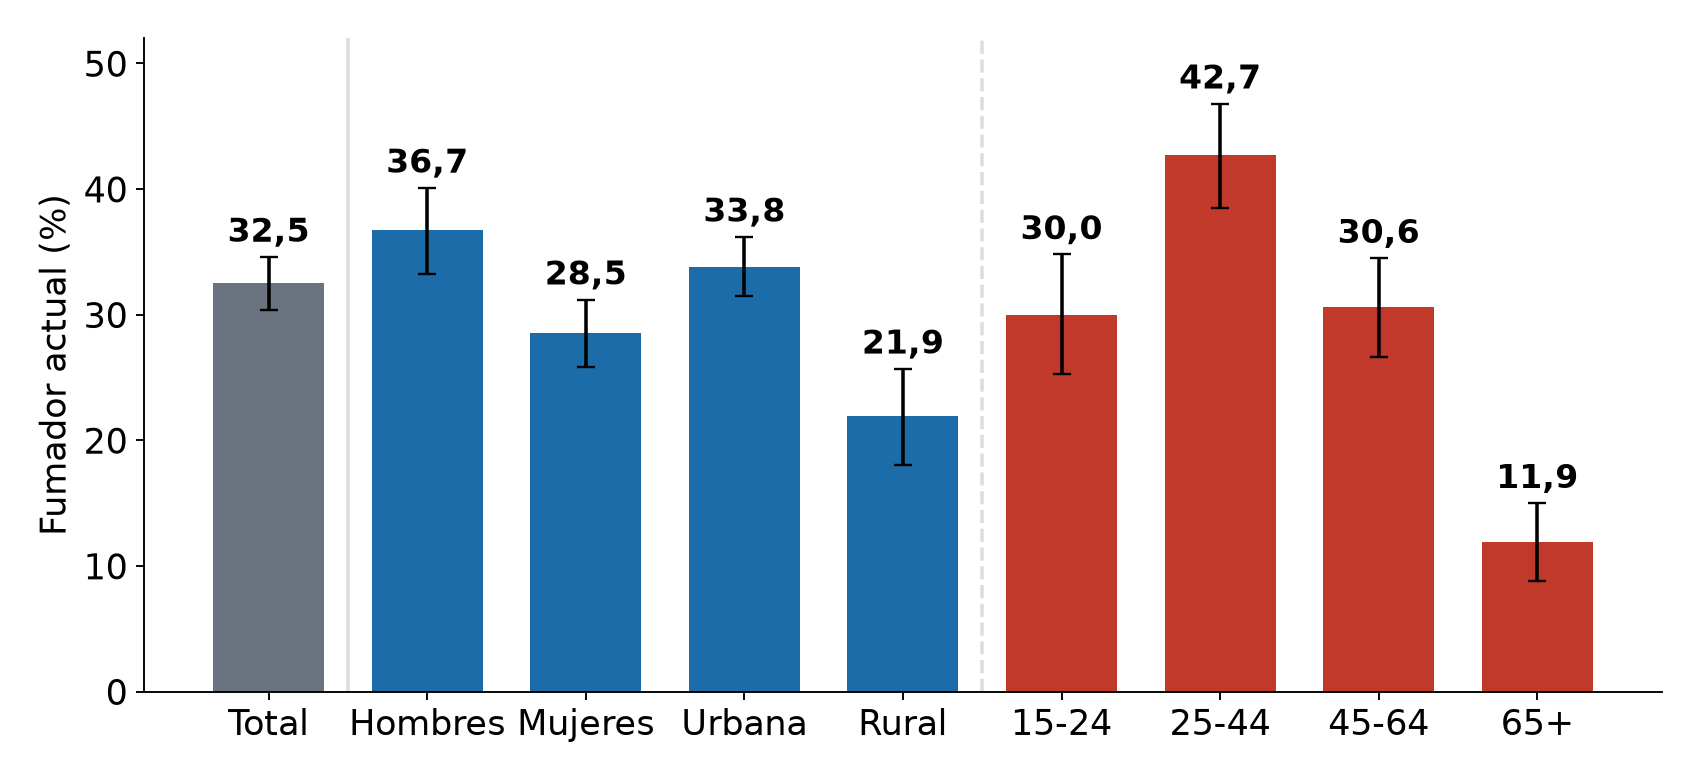
\includegraphics[width=.86\textwidth]{figs/fig_prevalencia.png}\\[.2em]
\begin{flushleft}\small
\dato{32,5\%} fuma actualmente (IC 95\% 30,4--34,6), unos \dato{4,7 millones} de personas.
Fuma a diario 24,5\%; ex fumador 25,3\%; nunca fumó 42,2\%.
\end{flushleft}
\fuente{ENS 2016-17, ponderado con estratos y conglomerados. Barras = prevalencia; líneas = IC 95\%.}
\end{frame}

% ------------------------------------------------------------------
\begin{frame}{Resultado 2 — Exposición al humo ajeno}
\begin{columns}[c]
\column{.55\textwidth}
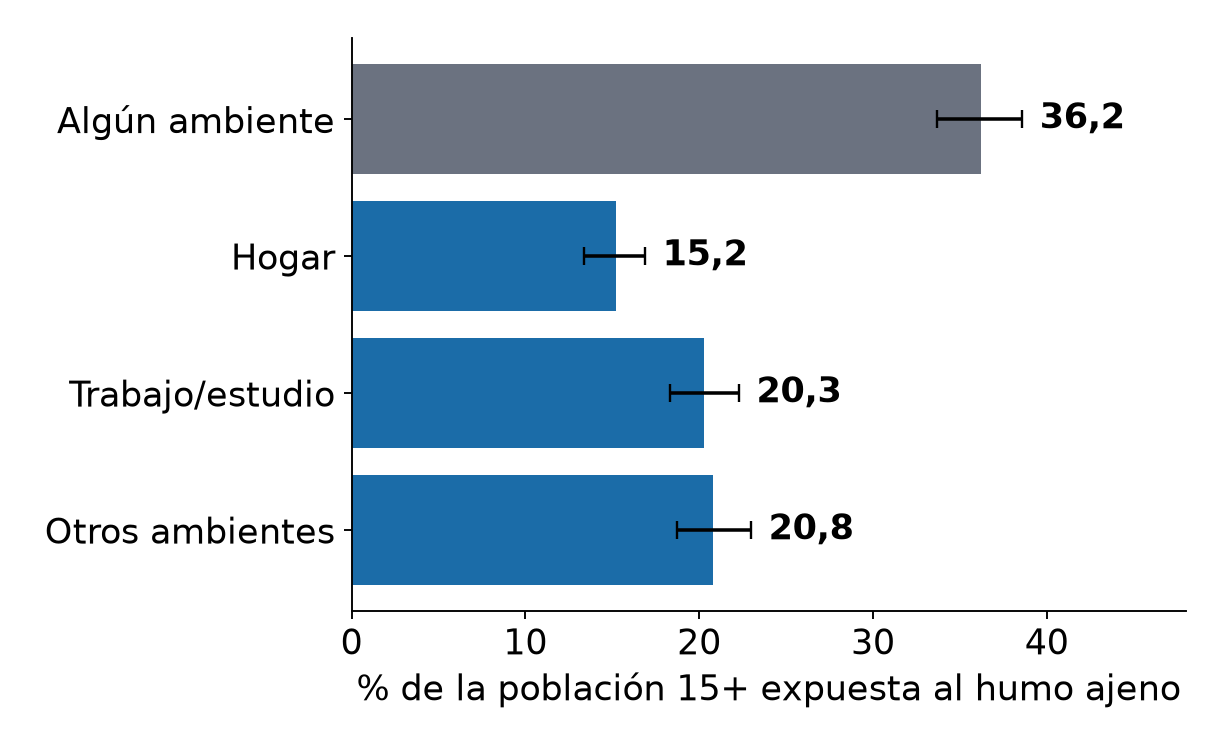
\includegraphics[width=\textwidth]{figs/fig_pasivo.png}
\column{.45\textwidth}
\begin{block}{Fumador pasivo}
No fuma actualmente y está expuesto:\\[.3em]
{\Large\dato{25,9\%}}\\
(IC 95\% 23,1--28,6)
\end{block}
\small
Los más expuestos: jóvenes de 15 a 24 años (48,3\% en algún ambiente) y hombres (43,0\% frente a 29,6\%).
\end{columns}
\fuente{Gráfico: población total de 15 años y más. Definición de exposición propia (hora $>0$), autorreportada.}
\end{frame}

% ------------------------------------------------------------------
\begin{frame}{Resultado 3 — ¿Fumar protege? Un resultado engañoso}
\begin{columns}[T]
\column{.5\textwidth}
\textbf{Mirada ingenua}\par\vspace{.3em}
\begin{tabular}{@{}lr@{}}
Fallecidos entre fumadores & 5,6\%\\
Fallecidos entre no fumadores & 9,9\%\\
HR sin ajustar & \textcolor{gris}{0,66}
\end{tabular}
\column{.5\textwidth}
\textbf{Qué estaba pasando}\par\vspace{.3em}
\begin{tabular}{@{}lr@{}}
Edad media fumadores & 43,1 años\\
Edad media no fumadores & 51,2 años
\end{tabular}
\end{columns}
\vspace{1em}
\begin{alertblock}{Confusión por edad}
Los fumadores son más jóvenes, y los mayores mueren más. Hay que \alert{comparar a personas de la misma edad}.
\end{alertblock}
\end{frame}

% ------------------------------------------------------------------
\begin{frame}{Resultado 4 — Ajustando por edad y sexo}
\centering
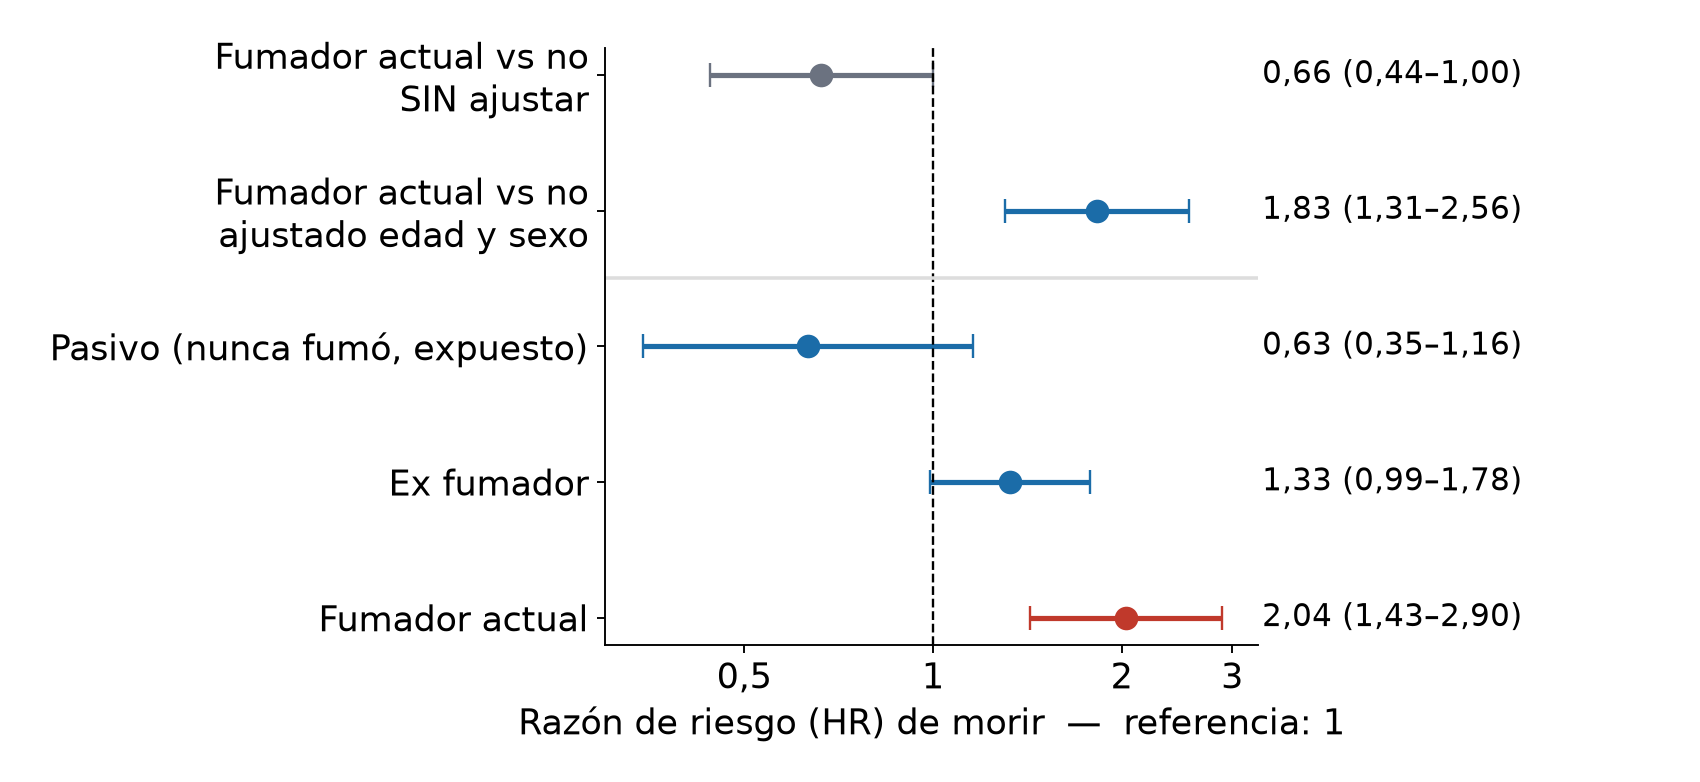
\includegraphics[width=.9\textwidth]{figs/fig_forest.png}
\begin{flushleft}\small
Fumadores actuales: unas \dato{2 veces} el riesgo de morir (HR 2,04; IC 95\% 1,43--2,90). Referencia: nunca fumó y sin exposición.
\end{flushleft}
\fuente{Modelo de Cox ponderado, errores estándar agrupados por conglomerado. 6.233 personas, 539 muertes.}
\end{frame}

% ------------------------------------------------------------------
\begin{frame}{Mirar las curvas de supervivencia}
\centering
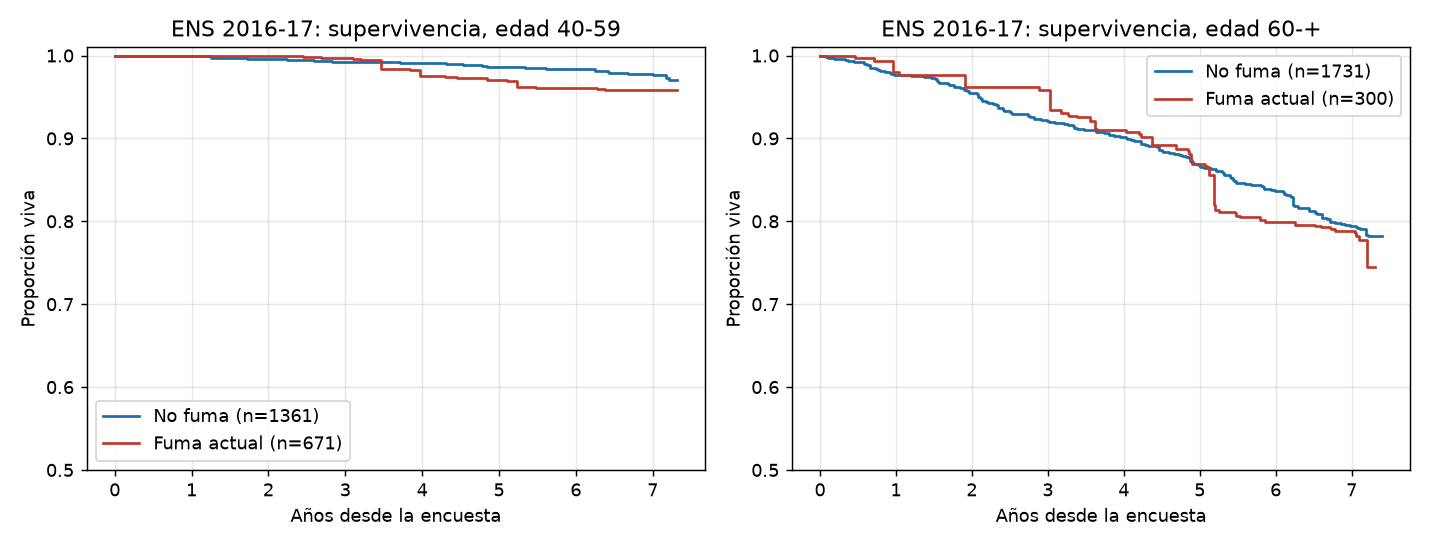
\includegraphics[width=.92\textwidth]{figs/fig_km.png}
\begin{flushleft}\small
Dentro de un mismo grupo de edad se compara mejor: en los de 40 a 59 años las curvas de fumadores caen antes; en los de 60 y más se superponen (pocos fumadores y sobrevivientes seleccionados).
\end{flushleft}
\fuente{Kaplan--Meier ponderado. Ejes recortados para ver la diferencia.}
\end{frame}

% ------------------------------------------------------------------
\begin{frame}{Fumadores pasivos: cuidado con la conclusión}
\begin{columns}[T]
\column{.5\textwidth}
\begin{tabular}{@{}lrr@{}}
\toprule
 & \textbf{Personas} & \textbf{Muertes}\\
\midrule
Referencia & 2.544 & 245\\
\alert{Pasivo} & \alert{473} & \alert{24}\\
Ex fumador & 1.456 & 172\\
Fumador actual & 1.760 & 98\\
\bottomrule
\end{tabular}
\column{.5\textwidth}
HR pasivo: \dato{0,63} (IC 95\% 0,35--1,16)
\vspace{.5em}
\begin{itemize}
  \item No es significativo.
  \item Con \alert{24 muertes} el estudio no tiene poder para detectar un efecto moderado.
\end{itemize}
\end{columns}
\vspace{.8em}
\begin{alertblock}{Cómo redactarlo}
«No encontramos asociación»~$\neq$~«el tabaco pasivo no hace daño». \alert{Ausencia de evidencia no es evidencia de ausencia.}
\end{alertblock}
\end{frame}

% ------------------------------------------------------------------
\begin{frame}{¿Y si fueron los enfermos quienes dejaron de fumar?}
\textbf{Causalidad inversa.} Personas ya enfermas pueden haber dejado de fumar o morir pronto por una enfermedad previa.\par
\vspace{.8em}
\textbf{Análisis de sensibilidad:} repetir el modelo \alert{sin las muertes de los primeros 2 años}.
\vspace{.5em}
\begin{center}
\begin{tabular}{lr}
\toprule
\textbf{Modelo} & \textbf{HR fumador actual}\\
\midrule
Ajustado por edad y sexo & 1,83 (1,31--2,56)\\
Excluyendo muertes $<$ 2 años & \dato{2,00} (1,39--2,88)\\
\bottomrule
\end{tabular}
\end{center}
\vspace{.5em}
La conclusión se mantiene: el resultado \textbf{no depende} de las muertes tempranas.
\end{frame}

% ------------------------------------------------------------------
\begin{frame}{Limitaciones que debemos declarar}
\begin{enumerate}
  \item \textbf{Tabaco medido una sola vez}, al inicio del seguimiento.
  \item \textbf{Pocas muertes} en algunos grupos (pasivos): poca potencia.
  \item \textbf{Exposición pasiva autorreportada}, sin biomarcador (cotinina) y con definición propia.
  \item \textbf{Confusión residual}: nivel socioeconómico, alcohol, enfermedades previas.
  \item \textbf{Errores estándar de mortalidad:} agrupan por conglomerado pero no incorporan el estrato.
  \item \textbf{Asociación, no causa}: es un estudio observacional.
\end{enumerate}
\end{frame}

% ------------------------------------------------------------------
\begin{frame}{De los números a un artículo}
\begin{columns}[T]
\column{.5\textwidth}
\textbf{Para reportar (STROBE)}
\begin{itemize}
  \item Diseño y población.
  \item Definiciones exactas.
  \item Estadística: pesos, diseño, ajustes.
  \item IC 95\% y \alert{n de eventos}.
  \item Sensibilidad y limitaciones.
\end{itemize}
\column{.5\textwidth}
\textbf{Antes de empezar}
\begin{itemize}
  \item Escribir el \textbf{protocolo} y el plan de análisis \alert{antes} de mirar resultados.
  \item Consultar al comité de ética.
  \item Citar la fuente y enviar copia al Minsal.
\end{itemize}
\end{columns}
\end{frame}

% ------------------------------------------------------------------
\begin{frame}{Ahora les toca a ustedes}
\textbf{Cuaderno de trabajo:} \texttt{taller\_tabaco\_PARTICIPANTES.ipynb}\par\vspace{.6em}
\begin{tabular}{@{}rp{.78\textwidth}@{}}
\dato{1} & Explorar la base\\
\dato{2--3} & Prevalencia de fumadores y de fumadores pasivos\\
\dato{4--5} & El resultado engañoso y el ajuste por edad\\
\dato{6} & Activos, ex y pasivos: ¿qué muestra el número de muertes?\\
\dato{7--8} & Sensibilidad y curvas de supervivencia\\
\dato{9} & Redactar el párrafo de resultados
\end{tabular}
\vspace{.8em}
\begin{block}{Para discutir}
¿Cambia el resultado si definimos «fumador pasivo» con otro umbral? ¿Qué otra pregunta podríamos responder con esta base?
\end{block}
\end{frame}

% ------------------------------------------------------------------
\begin{frame}[standout]
Gracias
\end{frame}

\appendix
\begin{frame}{Fuentes}
\small
\begin{itemize}
  \item Ministerio de Salud de Chile, Departamento de Epidemiología. \textit{Encuesta Nacional de Salud 2016-2017}: base de datos y manual de uso. \texttt{epi.minsal.cl/bases-de-datos}
  \item Base «ENS + Defunción (Mortalidad) 2023», mismo sitio.
  \item Condiciones de uso: \texttt{epi.minsal.cl/condiciones-de-uso}
  \item von Elm E. et al. \textit{STROBE statement.} (lista de verificación para estudios observacionales).
\end{itemize}
\vspace{.5em}
\textbf{Nota metodológica:} resultados calculados por nosotros con los datos públicos. La prevalencia de 32,5\% no fue contrastada con el informe oficial.
\end{frame}

\end{document}
